\section{Experimento}
\subsection{Conjunto de datos}

\begin{frame}{DAOs census\footnote{\footcite{tfm-dataset-text}}}
\begin{columns}
\column{.35\linewidth}    
    \begin{itemize}
        \item 30~000 DAOs
        \item 5 millones de votantes
        \item 22 millones de votos emitidos
        \item 180 mil propuestas
    \end{itemize}
\column{.65\linewidth}
\pause
\begin{table}[]
    \centering
    \small
    \begin{tabular}{l|r|r|r|r}
        \textbf{DAO} & 
        \textbf{Props.} & 
        \textbf{Usu.} & 
        \textbf{Vot.} &
        \textperthousand \textbf{Dns.} \\
        \hline
DEAD Foundations      & 5 591 & 3k   & 18k  & 1.83 \\ 
PancakeSwap           & 2 691 & 130k & 533k & 3.05 \\
\textit{Decentraland} & 2 060 & 7k   & 117k & 15.47 \\
AAVE                  & 1 140 & 87k  & 2.3M & 47.28 \\
MetaCartel            &   934 & 200  & 3k   & 35.38 \\
    \end{tabular}
    \caption{Resumen de datos de algunas DAOs}
    \label{tab:my_label}
\end{table}
\end{columns}
\end{frame}

\begin{frame}{Decentraland}
\blfootnote{Fuente: Figuras 4.3 a 4.6 de la memoria}

\begin{itemize}
    \item El 50\% de los 7k usuarios han votado como mucho en 3 propuestas
    \item Las propuestas duran 7 o 14 días
    \item Media de 56 votos por propuesta
    \item Picos de hasta 70 propuestas
    \item Se suelen votar poco después (48 horas) de su fecha de creación
    \item Las propuestas no se crean uniformemente a lo largo del dia de la semana
\end{itemize}
\end{frame}

\subsection{Entrenamiento y validación}

\begin{frame}{División en entrenamiento y prueba}
    \begin{figure}
        \centering
        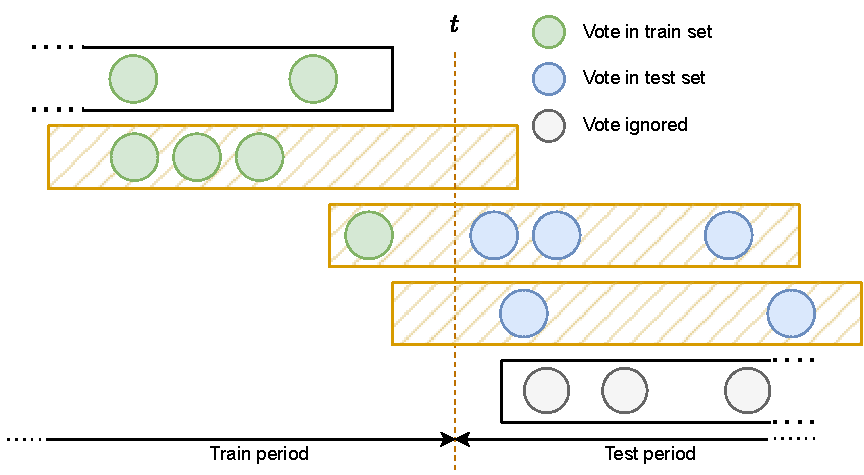
\includegraphics[height=55mm]{images/diagrams/rs-time-folds-evaluacion.drawio.pdf}
        % \caption{Ejemplo de split en \textit{entrenamiento} y \textit{prueba}}
    \end{figure}
\end{frame}


\begin{frame}{Métricas utilizadas}   
\begin{columns}
\column{.4\linewidth}
    \begin{itemize}
        \item precision@k
        \item recall@k
        \item nDCG@k
        \item MAP@k
    \end{itemize}
\column{.6\linewidth}
    \pause
    \centering
    \begin{alertblock}{Cuidado con $k>\left|\text{items rel. en top k}\right|$}
    \begin{equation}
        precision@k=\frac{\left|\text{items rel. en top k}\right|}{k}
    \end{equation}
    \end{alertblock}
\end{columns}
\end{frame}

\begin{frame}{La línea base \textit{OpenPop}}
\begin{columns}
    \column{.5\linewidth}
    \begin{alertblock}{Most Popular no tiene en cuenta:}
    \begin{itemize}
        \item La popularidad en ese momento dado
        \item Si el ítems estaba disponible
        \item Que la prop. puede estar cerrada
    \end{itemize}
    \end{alertblock}
    \column{.5\linewidth}
    \pause
    \begin{exampleblock}{OpenPop}
        Dado un instante $t$, recomendar la propuesta \textbf{abierta} más votada en ese momento siempre que el usuario no haya votado ya en ella.
    \end{exampleblock}
\end{columns}

\blfootnote{\footcite{rendle_difficulty_2019}}
\blfootnote{\footcite{ji_re-visit_2020}}
\end{frame}
